\documentclass{beamer}
\usepackage[utf8]{inputenc}
\usepackage{graphicx, epsfig}
\usepackage{amsmath,mathrsfs,amsfonts,amssymb}
\usepackage{floatflt}
\usepackage{epic,ecltree}
\usepackage{mathtext}
\usepackage{fancybox}
\usepackage{fancyhdr}
\usepackage{multirow}
\usepackage{enumerate}
\usepackage{epstopdf}
\usepackage{multicol}
\usepackage{algorithm}
\usepackage[noend]{algorithmic}
\usepackage{tikz}
\usepackage{blindtext}
\usepackage{multido}
\usetheme{default}%{Singapore}%{Warsaw}%{Warsaw}%{Darmstadt}
\usecolortheme{default}

\setbeamerfont{title}{size=\Huge}
\setbeamertemplate{footline}[frame number]{}

\setbeamertemplate{section in toc}[sections numbered]

\makeatletter
\newcommand\HUGE{\@setfontsize\Huge{35}{40}}
\makeatother    

\setbeamerfont{title}{size=\HUGE}
\beamertemplatenavigationsymbolsempty

\usetikzlibrary{arrows,shapes,positioning,shadows,trees}

\newcommand\myfootnote[1]{%
  \vspace{-0.5cm}%
  \tikz[remember picture,overlay]
  \draw (current page.south west) +(1in + \oddsidemargin,0.5em)
  node[anchor=south west,inner sep=0pt]{\parbox{\textwidth}{%
      \rlap{\rule{10em}{0.4pt}}\raggedright\scriptsize \textit{#1}}};}

\newcommand\myfootnotewithlink[2]{%
  \vspace{-0.5cm}%
  \tikz[remember picture,overlay]
  \draw (current page.south west) +(1in + \oddsidemargin,0.5em)
  node[anchor=south west,inner sep=0pt]{\parbox{\textwidth}{%
      \rlap{\rule{10em}{0.4pt}}\raggedright\scriptsize\href{#1}{\textit{#2}}}};}

\AtBeginSection[]
      {
      	\begin{frame}{Outline}
      		\tableofcontents[currentsection]
      	\end{frame}
      }
      \AtBeginSubsection[]{
      	\begin{frame}{Outline}
      		\tableofcontents[currentsection,currentsubsection]
      	\end{frame}
}

\newcounter{noscounter} % Используется для nextonslide команды (обнуляется только на новом слайде)
\newcounter{pcounter} % Используется для pause команды (обнуляется после использования eqpause)
\newcounter{diffcounter} % Считает количество pause после формулы

\newcommand{\nextonslide}[1]{%
  \stepcounter{noscounter}% Прибавляем счетчик nextonslide
  \stepcounter{pcounter}% Прибавляем счетчик pause
  \stepcounter{diffcounter}% Прибавляем счетчик diffcounter
  \onslide<\value{noscounter}->{#1}% Отображаем аргумент в скобках на слайде с номером noscounter
}
\newcommand{\resetonslide}{%
    \setcounter{noscounter}{1}% Сбрасываем счетчик nextonslide
    \setcounter{pcounter}{1}% Сбрасываем счетчик pause
    \setcounter{diffcounter}{0}% Сбрасываем счетчик diffcounter
}

\newcommand{\eqpause}{%
  \multido{\i=1+1}{\value{pcounter}}{\pause}% Повторяем pcounter раз команду pause
  \stepcounter{noscounter}% Прибавляем счетчик nextonslide
  \setcounter{pcounter}{1}% Сбрасываем счетчик pause
}

\newcommand{\eqpausediff}{% Вспомогательная команда, запускается автоматически после формул
  \multido{\i=1+1}{\value{diffcounter}}{\pause}% Повторяем diffcounter раз команду pause
  \addtocounter{pcounter}{-\value{diffcounter}}% Вычитаем из pcounter количество сделанных pause
  \setcounter{diffcounter}{0}% Сбрасываем счетчик diffcounter
}

\newcommand\AtEndBoth[2]{% Применяем команду к multline и multline*
  \AtEndEnvironment{#1}{#2}%
  \AtEndEnvironment{#1*}{#2}%
}

\AtEndBoth{align}{\eqpausediff}
\AtEndBoth{equation}{\eqpausediff}
\AtEndBoth{multline}{\eqpausediff}

\addtobeamertemplate{frametitle}{\resetonslide}{}% На каждом слайде сбрасываем счетчики

% latin bold lower
\newcommand{\ba}{\mathbf{a}} 
\newcommand{\bc}{\mathbf{c}} 
\newcommand{\be}{\mathbf{e}} 
\newcommand{\bff}{\mathbf{f}} % \bf - for bold type
\newcommand{\bg}{\mathbf{g}} 
\newcommand{\bh}{\mathbf{h}} 
\newcommand{\bp}{\mathbf{p}} 
\newcommand{\bq}{\mathbf{q}} 
\newcommand{\bt}{\mathbf{t}} 
\newcommand{\bs}{\mathbf{s}} 
\newcommand{\bu}{\mathbf{u}} 
\newcommand{\bv}{\mathbf{v}} 
\newcommand{\bw}{\mathbf{w}} 
\newcommand{\bx}{\mathbf{x}} 
\newcommand{\by}{\mathbf{y}} 
\newcommand{\bz}{\mathbf{z}} 

% latin bold upper
\newcommand{\bA}{\mathbf{A}} 
\newcommand{\bB}{\mathbf{B}} 
\newcommand{\bC}{\mathbf{C}} 
\newcommand{\bG}{\mathbf{G}} 
\newcommand{\bI}{\mathbf{I}} 
\newcommand{\bJ}{\mathbf{J}} 
\newcommand{\bL}{\mathbf{L}} 
\newcommand{\bM}{\mathbf{M}} 
\newcommand{\bP}{\mathbf{P}}
\newcommand{\bQ}{\mathbf{Q}} 
\newcommand{\bR}{\mathbf{R}} 
\newcommand{\bT}{\mathbf{T}} 
\newcommand{\bU}{\mathbf{U}} 
\newcommand{\bV}{\mathbf{V}} 
\newcommand{\bW}{\mathbf{W}} 
\newcommand{\bX}{\mathbf{X}} 
\newcommand{\bY}{\mathbf{Y}} 
\newcommand{\bZ}{\mathbf{Z}} 

% latin cal upper
\newcommand{\cF}{\mathcal{F}} 
\newcommand{\cG}{\mathcal{G}} 
\newcommand{\cI}{\mathcal{I}} 
\newcommand{\cL}{\mathcal{L}} 
\newcommand{\cM}{\mathcal{M}} 
\newcommand{\cN}{\mathcal{N}} 
\newcommand{\cP}{\mathcal{P}} 
\newcommand{\cS}{\mathcal{S}} 
\newcommand{\cT}{\mathcal{T}} 
\newcommand{\cW}{\mathcal{W}} 
\newcommand{\cX}{\mathcal{X}} 
\newcommand{\cZ}{\mathcal{Z}} 

% latin bb upper
\newcommand{\bbE}{\mathbb{E}} 
\newcommand{\bbI}{\mathbb{I}} 
\newcommand{\bbP}{\mathbb{P}} 
\newcommand{\bbR}{\mathbb{R}} 

% greek bold lower
\newcommand{\bepsilon}{\boldsymbol{\epsilon}} 
\newcommand{\btheta}{\boldsymbol{\theta}} 
\newcommand{\blambda}{\boldsymbol{\lambda}} 
\newcommand{\bpi}{\boldsymbol{\pi}} 
\newcommand{\bmu}{\boldsymbol{\mu}} 
\newcommand{\bsigma}{\boldsymbol{\sigma}} 
\newcommand{\bphi}{\boldsymbol{\phi}} 

% greek bold upper
\newcommand{\bSigma}{\boldsymbol{\Sigma}} 

\DeclareMathOperator*{\argmin}{arg\,min}
\DeclareMathOperator*{\argmax}{arg\,max}
\newcommand{\createdgmtitle}[1]{\title[\hbox to 56mm{Deep Generative Models  \hfill\insertframenumber\,/\,\inserttotalframenumber}]
	{\vspace{1cm} \\ \textbf{Deep Generative Models} \\ {\Huge Lecture #1}}
	\author{Roman Isachenko}
	\institute{
		Moscow Institute of Physics and Technology \\
		Yandex School of Data Analysis
	}
	\date{2025, Autumn}
}
\createdgmtitle{13}

%--------------------------------------------------------------------------------
\begin{document}
%--------------------------------------------------------------------------------
\begin{frame}[noframenumbering,plain]
\titlepage
\end{frame}
%=======
\begin{frame}{Recap of Previous Lecture}
	\vspace{-0.3cm}
	\[
		d\bx = \bff(\bx, t) dt + g(t) d \bw
	\]
	\vspace{-0.3cm}
	\begin{block}{Variance Exploding SDE (NCSN)}
		\vspace{-0.5cm}
		\[
			d \bx = \sqrt{\frac{ d [\sigma^2(t)]}{dt}} \cdot d \bw, \quad \bff(\bx, t) = 0, \quad g(t) = \sqrt{\frac{ d [\sigma^2(t)]}{dt}} 
		\]
		The variance grows since $\sigma(t)$ is a monotonically increasing function.
	\end{block}
	\begin{block}{Variance Preserving SDE (DDPM)}
		\vspace{-0.3cm}
		\[
			d \bx = - \frac{1}{2} \beta(t) \bx(t) dt + \sqrt{\beta(t)} \cdot d \bw
		\]
		\[
			\bff(\bx, t) = - \frac{1}{2} \beta(t) \bx(t) , \quad g(t) = \sqrt{\beta(t)} 
		\]
		The variance is preserved if $\bx(0)$ has unit variance.
	\end{block}
	\myfootnotewithlink{https://arxiv.org/abs/2011.13456}{Song Y., et al. Score-Based Generative Modeling through Stochastic Differential Equations, 2020}
\end{frame}
%=======
\begin{frame}{Recap of Previous Lecture}
	\begin{block}{Discrete-Time Objective}
		\vspace{-0.3cm}
		\[
			\bbE_{\pi(\bx_0)} \bbE_{t \sim U\{1, T\}} \bbE_{q(\bx_t | \bx_0)}\bigl\| \bs_{\btheta, t}(\bx_t) - \nabla_{\bx_t} \log q(\bx_t | \bx_0) \bigr\|^2_2 
		\]
		\vspace{-0.5cm}
	\end{block}
	\begin{block}{Continuous-Time Objective}
		\vspace{-0.5cm}
		\[
			\bbE_{\pi(\bx(0))} \bbE_{t \sim U[0, 1]} \bbE_{q(\bx(t) | \bx(0))}\bigl\| \bs_{\btheta}(\bx(t), t) - {\color{teal}\nabla_{\bx(t)} \log q(\bx(t) | \bx(0))} \bigr\|^2_2 
		\]
		\vspace{-0.5cm}
	\end{block}
	\begin{block}{NCSN}
		\vspace{-0.3cm}
		\[
			q(\bx(t) | \bx(0)) = \cN\left(\bx(0), \left[\sigma^2(t) - \sigma^2(0)\right] \cdot \bI\right)
		\]
		\vspace{-0.5cm}
	\end{block}
	\begin{block}{DDPM}
		\vspace{-0.3cm}
		\[
			q(\bx(t) | \bx(0)) = \cN\left(\bx(0) e^{-\frac{1}{2} \int_0^t\beta(s)ds}, \left(1 - e^{- \int_0^t\beta(s)ds}\right) \cdot \bI\right)
		\]
		\vspace{-0.5cm}
	\end{block}
	
	\myfootnotewithlink{https://arxiv.org/abs/2011.13456}{Song Y., et al. Score-Based Generative Modeling through Stochastic Differential Equations, 2020}
\end{frame}
%=======
\begin{frame}{Recap of Previous Lecture}
	\begin{block}{Sampling}
		To sample, solve the reverse SDE using numerical solvers (\texttt{SDESolve}).
		\begin{figure}
			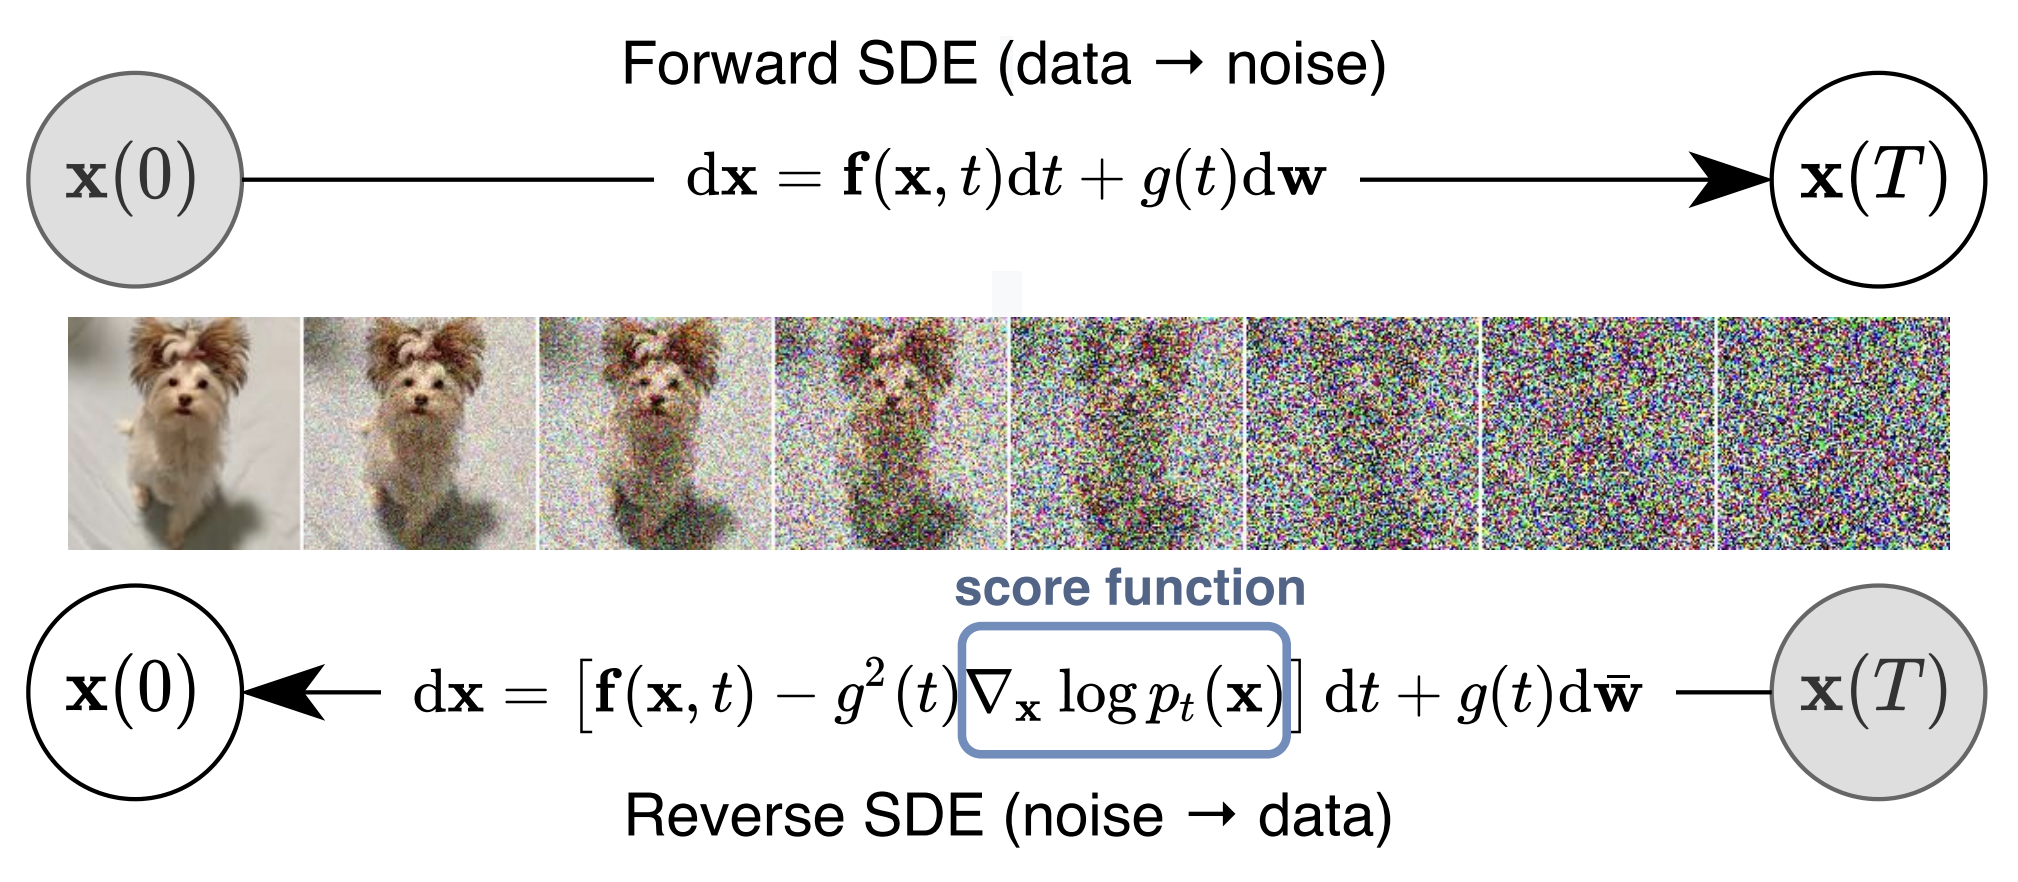
\includegraphics[width=0.8\linewidth]{figs/sbgm}
		\end{figure}
		\vspace{-0.5cm}
	\end{block}
	\begin{itemize}
		\item Discretizing the reverse SDE gives us ancestral sampling.
		\item If we use the probability flow ODE instead, then the reverse ODE yields DDIM sampling.
	\end{itemize}
	\myfootnotewithlink{https://arxiv.org/abs/2011.13456}{Song Y., et al. Score-Based Generative Modeling through Stochastic Differential Equations, 2020}
\end{frame}
%=======
\begin{frame}{Recap of Previous Lecture}
	Consider ODE dynamics $\bx(t)$ in the interval $t \in [0, 1]$ with $\bx_0 \sim p_0(\bx) = p(\bx)$, $\bx_1 \sim p_1(\bx) =  \pi(\bx)$.
	\[
		\frac{d \bx}{dt} = \bff (\bx, t),  \quad \text{with initial condition $\bx(0) = \bx_0$}.
	\]
	\vspace{-0.5cm}
	\begin{block}{KFP Theorem (Continuity Equation)}
		\vspace{-0.5cm}
		\[
			\frac{\partial p_t(\bx)}{\partial t} = - \text{div}\left(\bff(\bx, t) p_t(\bx)\right) \Leftrightarrow \frac{d \log p_t(\bx(t))}{d t} = - \text{tr} \left( \frac{\partial \bff(\bx(t), t)}{\partial \bx(t)} \right)
		\]
		\vspace{-0.3cm}
	\end{block}
	Solving the continuity equation using the adjoint method is complicated and unstable.
	\begin{block}{Flow Matching}
		\vspace{-0.3cm}
		\[
			\bbE_{t \sim U[0, 1]} \bbE_{\bx \sim p_t(\bx)}\left\| \bff(\bx, t) - \bff_{\btheta}(\bx, t) \right\|^2 \rightarrow \min_{\btheta}
		\]
		\vspace{-0.3cm}
	\end{block}
	\myfootnotewithlink{https://arxiv.org/abs/2210.02747}{Lipman Y., et al. Flow Matching for Generative Modeling, 2022}
\end{frame}
%=======
\begin{frame}{Recap of Previous Lecture}
	\vspace{-0.3cm}
	Introduce the latent variable $\bz$:
	\[
		p_t(\bx) = \int p_t(\bx | \bz) p(\bz) d \bz 
	\]
	\vspace{-0.5cm}
	\[
		\frac{\partial p_t(\bx | \bz)}{\partial t} = - \text{div}\left(\bff(\bx, \bz, t) p_t(\bx | \bz)\right).
	\]
	\vspace{-0.3cm}
	\begin{itemize}
		\item $p_t(\bx | \bz)$ is a \textbf{conditional probability path}
		\item $\bff(\bx, \bz, t)$ is a \textbf{conditional vector field}
	\end{itemize}
	\[
		\frac{d\bx}{dt} = \bff(\bx, t) \quad \Rightarrow \quad \frac{d\bx}{dt} = \bff(\bx, \bz, t)
	\]
	\vspace{-0.5cm}
	\begin{block}{Theorem}
		The following vector field generates the probability path $p_t(\bx)$:
		\vspace{-0.2cm}
		\[
			\bff(\bx, t) = \bbE_{p_t(\bz | \bx)} \bff(\bx, \bz, t)  = {\color{teal}\int \bff(\bx, \bz, t)} \frac{\color{teal}p_t(\bx | \bz) p(\bz)}{p_t(\bx)} {\color{teal}d \bz}
		\]
		\vspace{-0.5cm}
	\end{block}
	\myfootnotewithlink{https://arxiv.org/abs/2302.00482}{Tong A., et al. Improving and Generalizing Flow-Based Generative Models with Minibatch Optimal Transport, 2023}
\end{frame}
%=======
\begin{frame}{Recap of Previous Lecture}
	\begin{block}{Flow Matching (FM)}
		\vspace{-0.5cm}
		\[
			\bbE_{t \sim U[0, 1]} \bbE_{\bx \sim p_t(\bx)}\left\| \bff(\bx, t) - \bff_{\btheta}(\bx, t) \right\|^2 \rightarrow \min_{\btheta}
		\]
		\vspace{-0.5cm}
	\end{block}
	\begin{block}{Conditional Flow Matching (CFM)}
		\vspace{-0.5cm}
		\[
			\bbE_{t \sim U[0, 1]} \bbE_{\bz \sim p(\bz)} \bbE_{\bx \sim p_t(\bx | \bz)}\left\| \bff(\bx, \bz, t) - \bff_{\btheta}(\bx, t) \right\|^2 \rightarrow \min_{\btheta}
		\]
		\vspace{-0.5cm}
	\end{block}
	\begin{block}{Theorem}
		If $\text{supp}(p_t(\bx)) = \bbR^m$, then the optimal value of the FM objective equals the optimum for CFM.
	\end{block}
	\begin{figure}
		\centering
		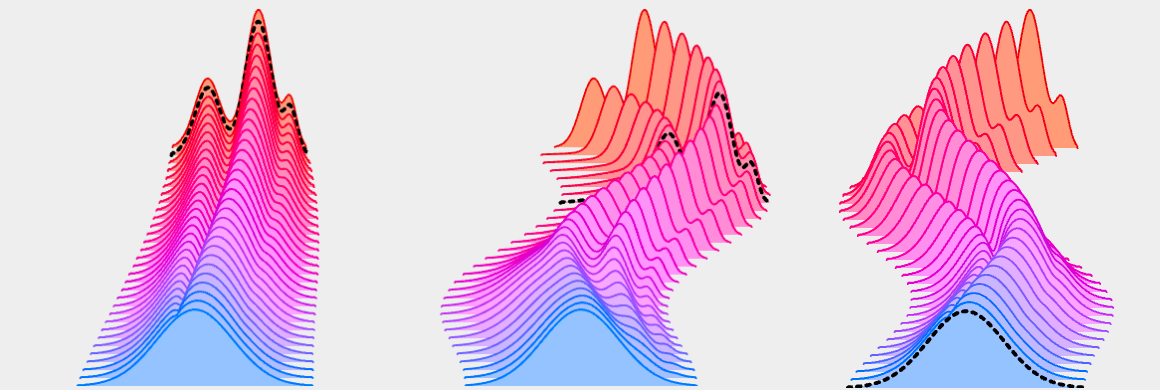
\includegraphics[width=0.8\linewidth]{figs/multiple_dynamics}
	\end{figure}
	\myfootnotewithlink{https://arxiv.org/abs/2302.00482}{Tong A., et al. Improving and Generalizing Flow-Based Generative Models with Minibatch Optimal Transport, 2023}
\end{frame}
%=======
\begin{frame}{Outline}
	\tableofcontents
\end{frame}
%=======
\section{Conditional Flow Matching}
%=======
\begin{frame}{Conditional Flow Matching}
	\[
		\bbE_{t \sim U[0, 1]} \bbE_{\bz \sim p(\bz)} \bbE_{\bx_t \sim p_t(\bx | \bz)}\left\| \bff(\bx_t, \bz, t) - \bff_{\btheta}(\bx_t, t) \right\|^2 \rightarrow \min_{\btheta}
	\]
	\[
		p(\bx) = \cN(0, \bI) = \bbE_{p(\bz)} p_0(\bx | \bz); \quad \pi(\bx) = \bbE_{p(\bz)} p_1(\bx | \bz).
	\]
	\vspace{-0.3cm}
	\begin{block}{Training}
		\begin{enumerate}
			\item Sample a time $t \sim U[0, 1]$ and $\bz \sim p(\bz)$.
			\item Draw $\bx_t \sim p_t(\bx | \bz)$.
			\item Compute the loss $ \cL = \left\| \bff(\bx_t, \bz, t) - \bff_{\btheta}(\bx_t, t) \right\|^2 $.
		\end{enumerate}
	\end{block}
	\begin{block}{Sampling}
		\begin{enumerate}
			\item Sample $\bx_0 \sim \cN(0, \bI)$.
			\item Solve the ODE to obtain $\bx_1$:
			\[
				\bx_1 = \texttt{ODESolve}_f(\bx_0, \btheta, t_0=0, t_1=1).
			\]
		\end{enumerate}
	\end{block}
	\myfootnotewithlink{https://arxiv.org/abs/2210.02747}{Lipman Y., et al. Flow Matching for Generative Modeling, 2022}
\end{frame}
%=======
\begin{frame}{Conditional Flow Matching}
	\vspace{-0.3cm}
	\[
		\bbE_{t \sim U[0, 1]} \bbE_{\bz \sim p(\bz)} \bbE_{\bx_t \sim p_t(\bx | \bz)}\left\| \bff(\bx_t, \bz, t) - \bff_{\btheta}(\bx_t, t) \right\|^2 \rightarrow \min_{\btheta}
	\]
	\vspace{-0.4cm}
	\begin{block}{Open Questions}
		\begin{itemize}
			\item How should we choose the conditioning latent variable $\bz$?
			\item How can we define $p_t(\bx | \bz)$ to enforce the constraints?
		\end{itemize}
	\end{block}
	\vspace{-0.3cm}
	\begin{block}{Gaussian Conditional Probability Path (Choice 2)}
		\vspace{-0.3cm}
		\[
			p_t(\bx | \bz) = \cN\left(\bmu_t(\bz), \bsigma_t^2(\bz)\right)
		\]
		\vspace{-0.5cm}
	\end{block}
	\begin{itemize}
		\item There are infinitely many vector fields that generate a particular probability path.
		\item Let's consider the following dynamics:
		\[
			\bx_t = \bmu_t(\bz) + \bsigma_t(\bz) \odot \bepsilon, \quad {\color{violet} \text{with fixed } \bepsilon \sim \cN(0, \bI)}
		\]
	\end{itemize}
	\myfootnotewithlink{https://arxiv.org/abs/2302.00482}{Tong A., et al. Improving and Generalizing Flow-Based Generative Models with Minibatch Optimal Transport, 2023}
\end{frame}
%=======
\begin{frame}{Flow Matching}
	\begin{block}{Gaussian Conditional Probability Path}
		\vspace{-0.3cm}
		\[
			p_t(\bx | \bz) = \cN\left(\bmu_t(\bz), \bsigma_t^2(\bz)\right); \quad \bx_t = \bmu_t(\bz) + \bsigma_t(\bz) \odot \bepsilon
		\]
		\vspace{-0.5cm}
	\end{block}
	\begin{block}{Theorem}
		\vspace{-0.3cm}
		\[
			\bff(\bx_t, \bz, t) =  \bmu_t'(\bz) + \frac{\bsigma_t'(\bz)}{\bsigma_t(\bz)} \odot (\bx_t - \bmu_t(\bz))
		\]
		\vspace{-0.3cm}
	\end{block}
	\vspace{-0.2cm}
	\begin{block}{Proof}
	\vspace{-0.2cm}
	\[
		\frac{d\bx_t}{dt} = \bff(\bx_t, \bz, t); \quad \bepsilon = \frac{1}{\bsigma_t(\bz)} \odot (\bx_t - \bmu_t(\bz))
	\]
	\[
		\frac{d\bx_t}{dt} = \bmu_t'(\bz) + \bsigma_t'(\bz) \odot \bepsilon =  \bmu_t'(\bz) + \frac{\bsigma_t'(\bz)}{\bsigma_t(\bz)} \odot (\bx_t - \bmu_t(\bz))
	\]
	\end{block}
	\myfootnotewithlink{https://arxiv.org/abs/2302.00482}{Tong A., et al. Improving and Generalizing Flow-Based Generative Models with Minibatch Optimal Transport, 2023}
\end{frame}
%=======
\section{Conical Gaussian Paths}
%=======
\begin{frame}{Endpoint Conditioning}
	\begin{block}{Conditional Flow Matching}
		\vspace{-0.3cm}
		\[
			\bbE_{t \sim U[0, 1]} \bbE_{\bz \sim p(\bz)} \bbE_{\bx_t \sim p_t(\bx | \bz)}\left\| \bff(\bx_t, \bz, t) - \bff_{\btheta}(\bx_t, t) \right\|^2 \rightarrow \min_{\btheta}
		\]
		\vspace{-0.3cm}
	\end{block}
	\begin{block}{Conditioning Latent Variable (Choice 1)}
		Let us choose $\bz = \bx_1$. Then $p(\bz) = p_1(\bx_1)$.
		\[
			p_t(\bx) = \int p_t(\bx | \bx_1) p_1(\bx_1) d \bx_1
		\]
	\end{block}
	We need to ensure the boundary constraints:
	\[
		\begin{cases}
			p(\bx) = \bbE_{p(\bz)} p_0(\bx | \bz); {\color{gray}(= \cN(0, \bI))} \\
			\pi(\bx) = \bbE_{p(\bz)} p_1(\bx | \bz)
		\end{cases}
		\quad \Rightarrow \quad 
		\begin{cases}
			p_0(\bx | \bx_1) = \cN(0, \bI); \\
			p_1(\bx | \bx_1) = \delta(\bx - \bx_1)
		\end{cases}
	\]
	\vspace{-0.3cm}
	\myfootnotewithlink{https://arxiv.org/abs/2210.02747}{Lipman Y., et al. Flow Matching for Generative Modeling, 2022}
\end{frame}
%=======
\begin{frame}{Conical Gaussian Paths}
	\[
		p_0(\bx | \bx_1) = \cN(0, \bI); \quad p_1(\bx | \bx_1) = \delta(\bx - \bx_1)
	\]
	
	\begin{block}{Gaussian Conditional Probability Path}
		\vspace{-0.5cm}
		\[
			p_t(\bx | \bx_1) = \cN\left(\bmu_t(\bx_1), \bsigma_t^2(\bx_1)\right); \quad \bx_t = \bmu_t(\bx_1) +  \bsigma_t(\bx_1) \odot {\color{olive}\bepsilon}
		\]
		\vspace{-0.6cm}
	\end{block}
	Let's consider straight conditional paths:	
	\[
		\begin{cases}
			\bmu_t(\bx_1) = t \bx_1 \\
			\bsigma_t(\bx_1) = 1 - t
		\end{cases}
		\quad \Rightarrow \quad 
		\begin{cases}
			p_t(\bx | \bx_1) = \cN\left(t \bx_1, (1-t)^2 \cdot \bI\right) \\
		 	\bx_t = t \bx_1 + (1 - t) {\color{olive}\bx_0}
	 \end{cases}
	\]
	\vspace{-0.3cm}
	\begin{figure}
		\centering
		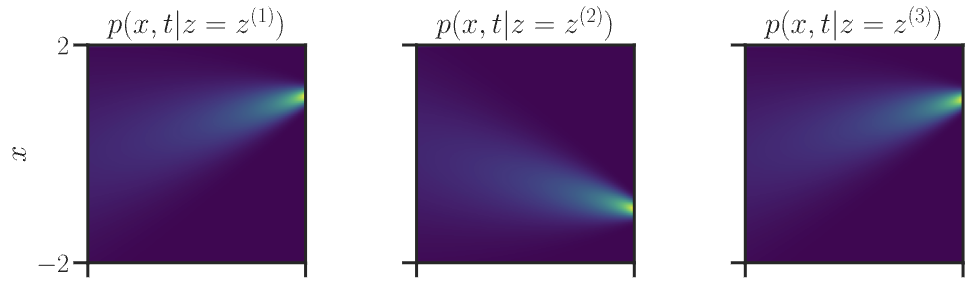
\includegraphics[width=\linewidth]{figs/conical_paths}
	\end{figure}
	\myfootnotewithlink{https://dl.heeere.com/conditional-flow-matching/blog/conditional-flow-matching}{image credit: A Visual Dive into Conditional Flow Matching}
\end{frame}
%=======
\begin{frame}{Conical Gaussian Paths}
	\[
		p_t(\bx | \bx_1) = \cN\left(t \bx_1, (1-t)^2 \bI\right); \quad {\color{teal}\bx_t = t \bx_1 + (1 - t) \bx_0}
	\]
	\vspace{-0.3cm}
	\begin{block}{Conditional Vector Field}
		\vspace{-0.3cm}
		\[
			 \frac{d\bx_t}{dt} = \bff(\bx_t, \bx_1, t) =  \bmu_t'(\bx_1) + \frac{\bsigma_t'(\bx_1)}{\bsigma_t(\bx_1)} \odot (\bx_t - \bmu_t(\bx_1))
		\]
		\vspace{-0.5cm}
		\begin{multline*}
			\bff(\bx_t, \bx_1, t) = \bx_1 - \frac{1}{1-t} \cdot (\bx_t - t \bx_1) = \frac{\bx_1 - {\color{teal}\bx_t}}{1-t} = \\
			= \frac{\bx_1 - {\color{teal}t \bx_1 - (1 - t) \bx_0}}{1-t} = \bx_1 - \bx_0
		\end{multline*}
		\vspace{-0.7cm}
	\end{block}
	\begin{minipage}[t]{0.55\columnwidth}
		\vspace{-0.7cm}
		\begin{figure}
			\centering
			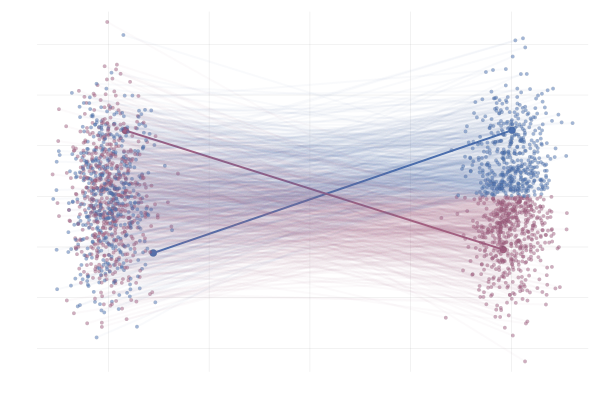
\includegraphics[width=0.9\linewidth]{figs/g2g-vector-field-samples-cond}
		\end{figure}
	\end{minipage}%
	\begin{minipage}[t]{0.45\columnwidth}
		The conditional vector field $\bff(\bx_t, \bx_1, t)$ defines straight lines between $\pi(\bx)$ and $\cN(0, \bI)$.
	\end{minipage}
	\myfootnotewithlink{https://mlg.eng.cam.ac.uk/blog/2024/01/20/flow-matching.html}{image credit: https://mlg.eng.cam.ac.uk/blog/2024/01/20/flow-matching.html}
\end{frame}
%=======
\begin{frame}{Conical Gaussian Paths}
	\vspace{-0.5cm}
	\begin{multline*}
		\bbE_{t \sim U[0, 1]} \bbE_{\bz \sim p(\bz)} \bbE_{\bx \sim p_t(\bx | \bz)}\left\| \bff(\bx, \bz, t) - \bff_{\btheta}(\bx, t) \right\|^2 = \\
		\bbE_{t \sim U[0, 1]} \bbE_{\bx_1 \sim \pi(\bx)} {\color{violet}\bbE_{\bx_t \sim p_t(\bx | \bx_1)}}\left\| \left(\frac{\bx_1 - \bx_t}{1-t}\right) - \bff_{\btheta}(\bx_t, t) \right\|^2 = \\
		\bbE_{t \sim U[0, 1]} \bbE_{\bx_1 \sim \pi(\bx)} {\color{violet}\bbE_{\bx_0 \sim \cN(0, \bI)}}\left\| (\bx_1 - \bx_0) - \bff_{\btheta}\left(t \bx_1 + (1 - t) \bx_0, t\right) \right\|^2
	\end{multline*}
	\vspace{-0.5cm}
	\begin{itemize}
		\item We fit straight lines between the noise distribution $p(\bx)$ and the data distribution $\pi(\bx)$.
		\item The \textbf{marginal} path $p_t(\bx)$ does not give straight lines.
	\end{itemize}
	\vspace{-0.3cm}
	\begin{minipage}[t]{0.5\columnwidth}
			\begin{figure}
				\centering
				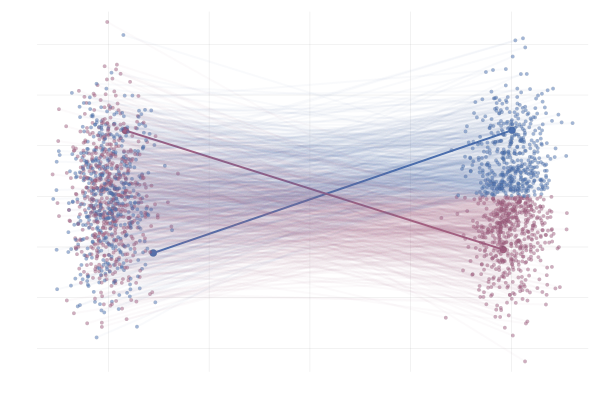
\includegraphics[width=\linewidth]{figs/g2g-vector-field-samples-cond}
			\end{figure}
		\end{minipage}%
		\begin{minipage}[t]{0.5\columnwidth}
			\begin{figure}
				\centering
				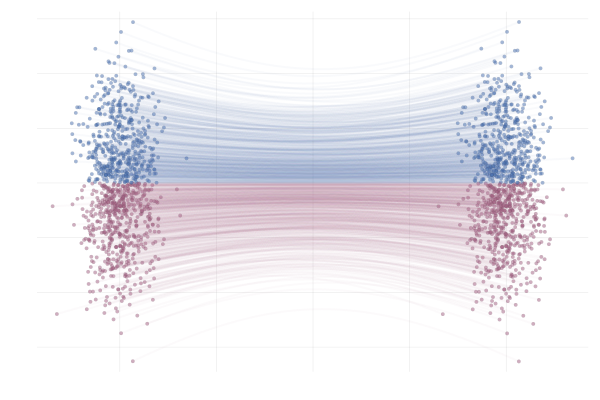
\includegraphics[width=\linewidth]{figs/g2g-forward_samples}
			\end{figure}
	\end{minipage}
	\myfootnotewithlink{https://arxiv.org/abs/2210.02747}{Lipman Y., et al. Flow Matching for Generative Modeling, 2022}
\end{frame}
%=======
\begin{frame}{Conditional Flow Matching}
	\vspace{-0.3cm}
	\[
	 \bbE_{t \sim U[0, 1]} \bbE_{\bx_1 \sim \pi(\bx)} \bbE_{\bx_0 \sim \cN(0, \bI)}\left\| (\bx_1 - \bx_0) - \bff_{\btheta}(\bx_t, t) \right\|^2  \rightarrow \min_{\btheta}
	\]
	\begin{block}{Training}
		\begin{enumerate}
			\item Sample $\bx_1 \sim \pi(\bx)$.
			\item Sample time $t \sim U[0, 1]$ and $\bx_0 \sim \cN(0, \bI)$.
			\item Obtain the noisy image $\bx_t = t \bx_1 + (1 - t) \bx_0$.
			\item Compute the loss $ \cL = \left\| (\bx_1 - \bx_0) - \bff_{\btheta}(\bx, t) \right\|^2 $.
		\end{enumerate}
	\end{block}
	\vspace{-0.3cm}
	\begin{block}{Sampling}
		\begin{enumerate}
			\item Sample $\bx_0 \sim \cN(0, \bI)$.
			\item Solve the ODE to obtain $\bx_1$:
			\[
				\bx_1 = \texttt{ODESolve}_f(\bx_0, \btheta, t_0=0, t_1=1)
			\]
		\end{enumerate}
	\end{block}
	\myfootnotewithlink{https://arxiv.org/abs/2210.02747}{Lipman Y., et al. Flow Matching for Generative Modeling, 2022}
\end{frame}
%=======
\section{Linear Interpolation}
%=======
\begin{frame}{Pair Conditioning}
	\begin{block}{Conditional Flow Matching}
		\vspace{-0.3cm}
		\[
			\bbE_{t \sim U[0, 1]} \bbE_{\bz \sim p(\bz)} \bbE_{\bx \sim p_t(\bx | \bz)}\left\| \bff(\bx, \bz, t) - \bff_{\btheta}(\bx, t) \right\|^2 \rightarrow \min_{\btheta}
		\]
		\vspace{-0.3cm}
	\end{block}
	\begin{block}{Conditioning Latent Variable (Choice 1)}
		Let us choose $\bz = (\bx_0, \bx_1)$. Then $p(\bz) = p (\bx_0, \bx_1) = p_0(\bx_0) p_1(\bx_1)$.
		\[
			p_t(\bx) = \int p_t(\bx | \bx_0, \bx_1) p_0(\bx_0) p_1(\bx_1) d \bx_0 d \bx_1
		\]
	\end{block}
	We must enforce boundary constraints:
	\[
		\begin{cases}
			p(\bx) = \bbE_{p(\bz)} p_0(\bx | \bz); {\color{gray}(= \cN(0, \bI))} \\
			\pi(\bx) = \bbE_{p(\bz)} p_1(\bx | \bz)
		\end{cases}
		\, \Rightarrow \, 
		\begin{cases}
			p_0(\bx | \bx_0, \bx_1) = \delta(\bx - \bx_0) \\
			p_1(\bx | \bx_0, \bx_1) = \delta(\bx - \bx_1)
		\end{cases}
	\]
	\vspace{-0.3cm}
	\myfootnotewithlink{https://arxiv.org/abs/2210.02747}{Lipman Y., et al. Flow Matching for Generative Modeling, 2022}
\end{frame}
%=======
\begin{frame}{Linear Interpolation}
	\[
		p_0(\bx | \bx_0, \bx_1) = \delta(\bx - \bx_0); \quad p_1(\bx | \bx_0, \bx_1) = \delta(\bx - \bx_1)
	\]
	
	\begin{block}{Gaussian Conditional Probability Path}
		\vspace{-0.5cm}
		{\small
		\[
			p_t(\bx | \bx_0, \bx_1) = \cN\left(\bmu_t(\bx_0, \bx_1), \bsigma_t^2(\bx_0, \bx_1)\right); \quad \bx_t = \bmu_t(\bx_0, \bx_1) +  \bsigma_t^2(\bx_0, \bx_1) \odot \bx_0
		\]
		}
		\vspace{-0.6cm}
	\end{block}
	Let's consider straight conditional paths:	
	\[
		\begin{cases}
			\bmu_t(\bx_1) = t \bx_1 + (1 - t) \bx_0 \\
			\bsigma_t(\bx_1) = \epsilon
		\end{cases}
		\quad \Rightarrow \quad 
		\begin{cases}
			p_0(\bx | \bx_0, \bx_1) = \delta(\bx - \bx_0) \\
			p_1(\bx | \bx_0, \bx_1) = \delta(\bx - \bx_1)
		\end{cases}
	\]
	\vspace{-0.3cm}
	\begin{figure}
		\centering
		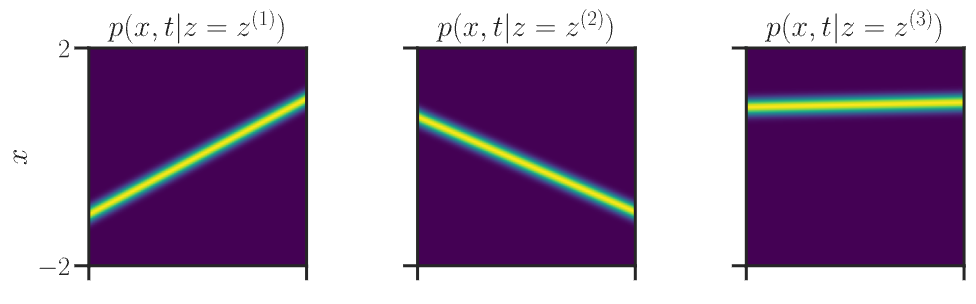
\includegraphics[width=\linewidth]{figs/linear_paths}
	\end{figure}
	\myfootnotewithlink{https://dl.heeere.com/conditional-flow-matching/blog/conditional-flow-matching}{image credit: A Visual Dive into Conditional Flow Matching}
\end{frame}
%=======
\begin{frame}{Flow Matching: Conical Paths vs. Linear Interpolation}
	\begin{minipage}[t]{0.5\columnwidth}
		\begin{align*}
			\bz & = \bx_1 \\
			p_t(\bx | \bx_1) &= \cN\left(t \bx_1, (1-t)^2 \bI\right) \\
			\bx_t &= t \bx_1 + (1 - t) \bx_0 
		\end{align*}
	\end{minipage}%
	\begin{minipage}[t]{0.5\columnwidth}
		\begin{align*}
			\bz & = (\bx_0, \bx_1) \\
			p_t(\bx | \bx_0, \bx_1) &= \cN\left(t \bx_1 + (1 - t) \bx_0, \epsilon^2 \bI\right) \\
			\bx_t &= t \bx_1 + (1 - t) \bx_0
		\end{align*}
	\end{minipage}
	\begin{figure}
		\centering
		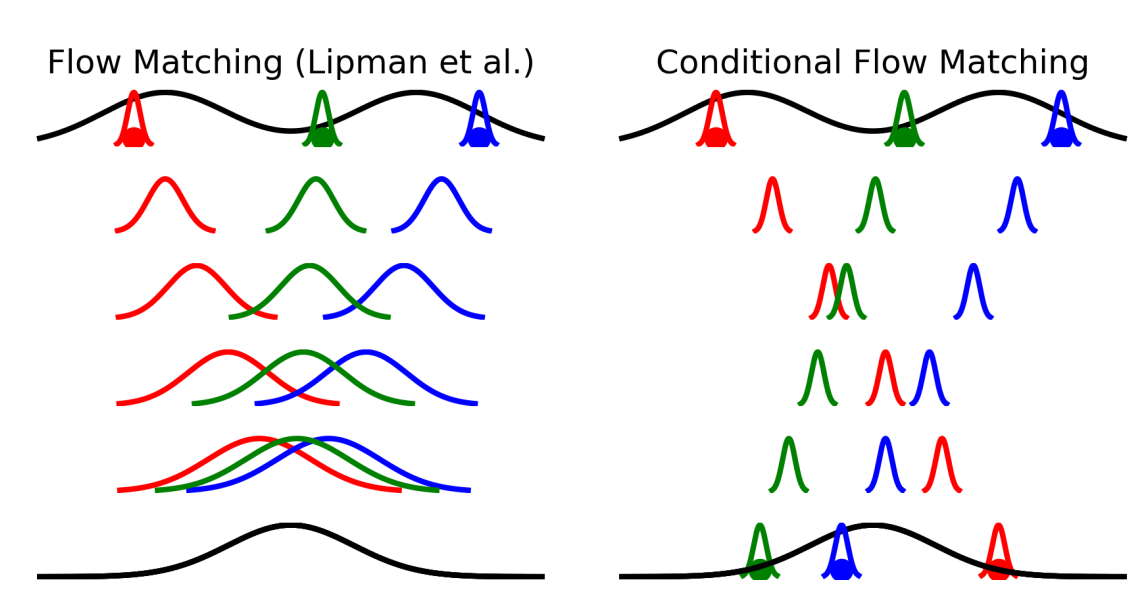
\includegraphics[width=0.8\linewidth]{figs/compare_conditionings}
	\end{figure}
	\myfootnotewithlink{https://arxiv.org/pdf/2302.00482}{Tong A., et al. Improving and Generalizing Flow-Based Generative Models with Minibatch Optimal Transport, 2023}
\end{frame}
%=======
\begin{frame}{Linear Interpolation}
	\vspace{-0.3cm}
	\[
		p_t(\bx | \bx_0, \bx_1) = \cN\left(t \bx_1 + (1 - t) \bx_0, \epsilon^2 \bI\right); \quad {\color{teal}\bx_t = t \bx_1 + (1 - t) \bx_0}
	\]
	\vspace{-0.5cm}
	\begin{block}{Conditional Vector Field}
		\vspace{-0.5cm}
		\[
			 \frac{d\bx_t}{dt} = \bff(\bx_t, \bx_0, \bx_1, t) =  \bmu_t'(\bx_0, \bx_1) + \frac{\bsigma_t'(\bx_0, \bx_1)}{\bsigma_t(\bx_0, \bx_1)} \odot (\bx_t - \bmu_t(\bx_0, \bx_1))
		\]
		\vspace{-0.5cm}
		\[
			\bff(\bx_t, \bx_0, \bx_1, t) = \bx_1 - \bx_0
		\]
		\vspace{-0.7cm}
	\end{block}
	\begin{block}{Conditional Flow Matching}
		\vspace{-0.7cm}
		\begin{multline*}
			\bbE_{t \sim U[0, 1]} \bbE_{\bz \sim p(\bz)} \bbE_{\bx \sim p_t(\bx | \bz)}\left\| \bff(\bx, \bz, t) - \bff_{\btheta}(\bx, t) \right\|^2 = \\
		 \bbE_{t \sim U[0, 1]} \bbE_{(\bx_0, \bx_1) \sim p(\bx_0, \bx_1)} \bbE_{\bx \sim p_t(\bx | \bx_0, \bx_1)} \left\| (\bx_1 - \bx_0) - \bff_{\btheta}(\bx_t, t) \right\|^2
		\end{multline*}
		\vspace{-0.5cm}
	\end{block}
	\begin{itemize}
		\item This yields the same procedure as for conical paths!
		\item Now, we do not require that $p_0(\bx)$ is necessarily $\cN(0, \bI)$.
	\end{itemize} 
	\myfootnotewithlink{https://arxiv.org/abs/2210.02747}{Lipman Y., et al. Flow Matching for Generative Modeling, 2022}
\end{frame}
%=======
\begin{frame}{Conditional Flow Matching}
	\begin{itemize}
		\item This conditioning allows us to transport any distribution $p_0(\bx)$ to any distribution $p_1(\bx)$.
		\item It's possible to apply this approach to paired tasks, e.g., style transfer.
	\end{itemize}
	\begin{block}{Training Procedure}
		\begin{enumerate}
			\item Sample $(\bx_0, \bx_1) \sim p(\bx_0, \bx_1)$.
			\item Sample time $t \sim U[0, 1]$.
			\item Compute the noisy image $\bx_t = t \bx_1 + (1 - t) \bx_0$.
			\item Compute the loss $ \cL = \left\| (\bx_1 - \bx_0) - \bff_{\btheta}(\bx, t) \right\|^2 $.
		\end{enumerate}
	\end{block}
	\vspace{-0.3cm}
	\begin{block}{Sampling}
		\begin{enumerate}
			\item Sample $\bx_0 \sim p_0(\bx)$.
			\item Solve the ODE to obtain $\bx_1$:
			\[
				\bx_1 = \texttt{ODESolve}_f(\bx_0, \btheta, t_0=0, t_1=1)
			\]
		\end{enumerate}
	\end{block}
	\myfootnotewithlink{https://arxiv.org/abs/2210.02747}{Lipman Y., et al. Flow Matching for Generative Modeling, 2022}
\end{frame}
%=======
\begin{frame}{Stable Diffusion 3: Scalable Flow Matching}
	\begin{figure}
		\centering
		\includegraphics[width=\linewidth]{figs/sd3}
	\end{figure}
	\myfootnotewithlink{https://arxiv.org/pdf/2403.03206}{Esser P., et al. Scaling Rectified Flow Transformers for High-Resolution Image Synthesis, 2024}
\end{frame}
%=======
\section{Link with Score-Based Models}
%=======
\begin{frame}{Score-Based Generative Models through SDEs}
	\vspace{-0.3cm}
	\begin{block}{Training}
		\vspace{-0.7cm}
		\[
			\bbE_{\pi(\bx(0))} \bbE_{t \sim U[0, 1]} \bbE_{q(\bx(t) | \bx(0))}\bigl\| \bs_{\btheta}(\bx(t), t) - {\color{teal}\nabla_{\bx(t)} \log q(\bx(t) | \bx(0))} \bigr\|^2_2 
		\]
		\vspace{-0.5cm}
	\end{block}
	\begin{block}{Variance Exploding SDE (NCSN)}
		\vspace{-0.3cm}
		\[
			q(\bx(t) | \bx(0)) = \cN\left(\bx(0), \left[\sigma^2(t) - \sigma^2(0)\right] \cdot \bI\right), \quad \sigma(0) =0
		\]
		\vspace{-0.5cm}
	\end{block}
	\begin{block}{Variance Preserving SDE (DDPM)}
		\vspace{-0.5cm}
		\[
			q(\bx(t) | \bx(0)) = \cN\left(\bx(0) \alpha(t), \left(1 - \alpha(t)^2\right) \cdot \bI\right); \quad \alpha(t) = e^{-\frac{1}{2} \int_0^t \beta(s) ds}
		\]
		\vspace{-0.5cm}
	\end{block}
	Flow matching uses reverse time direction:
	\[
		\textbf{NCSN: } p(\bx | \bx_1) = \cN\left(\bx_1, \sigma^2_{1-t} \cdot \bI\right)
	\]
	\vspace{-0.5cm}
	\[
		\textbf{DDPM: } p(\bx | \bx_1) = \cN\left(\alpha_{1-t} \bx_1, \left(1 - \alpha_{1-t}^2\right) \cdot \bI\right)
	\]
	\vspace{-0.5cm}
	\myfootnotewithlink{https://arxiv.org/abs/2210.02747}{Lipman Y., et al. Flow Matching for Generative Modeling, 2022}
\end{frame}
%=======
\begin{frame}{Flow Matching vs. Score-Based SDE Models}
	\begin{block}{Flow Matching Probability Path}
		\vspace{-0.3cm}
		\[
			p_t(\bx | \bx_1) = \cN\left(t \bx_1, (1-t)^2 \bI\right); \quad \bff(\bx, \bx_1, t) = \frac{\bx_1  - \bx}{1-t}
		\]
		\vspace{-0.3cm}
		\[
	 		\frac{d\bx}{dt} = \bff(\bx, \bx_1, t) =  \bmu_t'(\bx_1) + \frac{\bsigma_t'(\bx_1)}{\bsigma_t(\bx_1)} \odot (\bx - \bmu_t(\bx_1))
		\]
	\end{block}
	\begin{block}{Variance Exploding SDE Probability Path}
		\vspace{-0.3cm}
		\[
				p_t(\bx | \bx_1) = \cN\left(\bx_1, \sigma^2_{1-t}  \bI\right) \quad \Rightarrow \quad 
				\bff(\bx, \bx_1, t) = - \frac{\sigma'_{1-t}}{\sigma_{1-t}} (\bx - \bx_1)
		\]
		\vspace{-0.3cm}
	\end{block}
	\begin{block}{Variance Preserving SDE Probability Path}
		\vspace{-0.3cm}
		{\small
		\[
			p_t(\bx | \bx_1) = \cN\left(\alpha_{1-t}  \bx_1, (1 - \alpha^2_{1-t})  \bI \right)  \, \Rightarrow \, 
		\bff(\bx, \bx_1, t) = \frac{\alpha'_{1-t}}{1 - \alpha^2_{1-t}}\cdot \left(\alpha_{1-t}  \bx - \bx_1\right)
		\]
		}
	\end{block}
	\myfootnotewithlink{https://arxiv.org/abs/2210.02747}{Lipman Y., et al. Flow Matching for Generative Modeling, 2022}
\end{frame}
%=======
\begin{frame}{Flow Matching vs. Score-Based SDE Models}
	\begin{block}{Trajectories}
		\vspace{-0.3cm}
		\begin{figure}
			\centering
			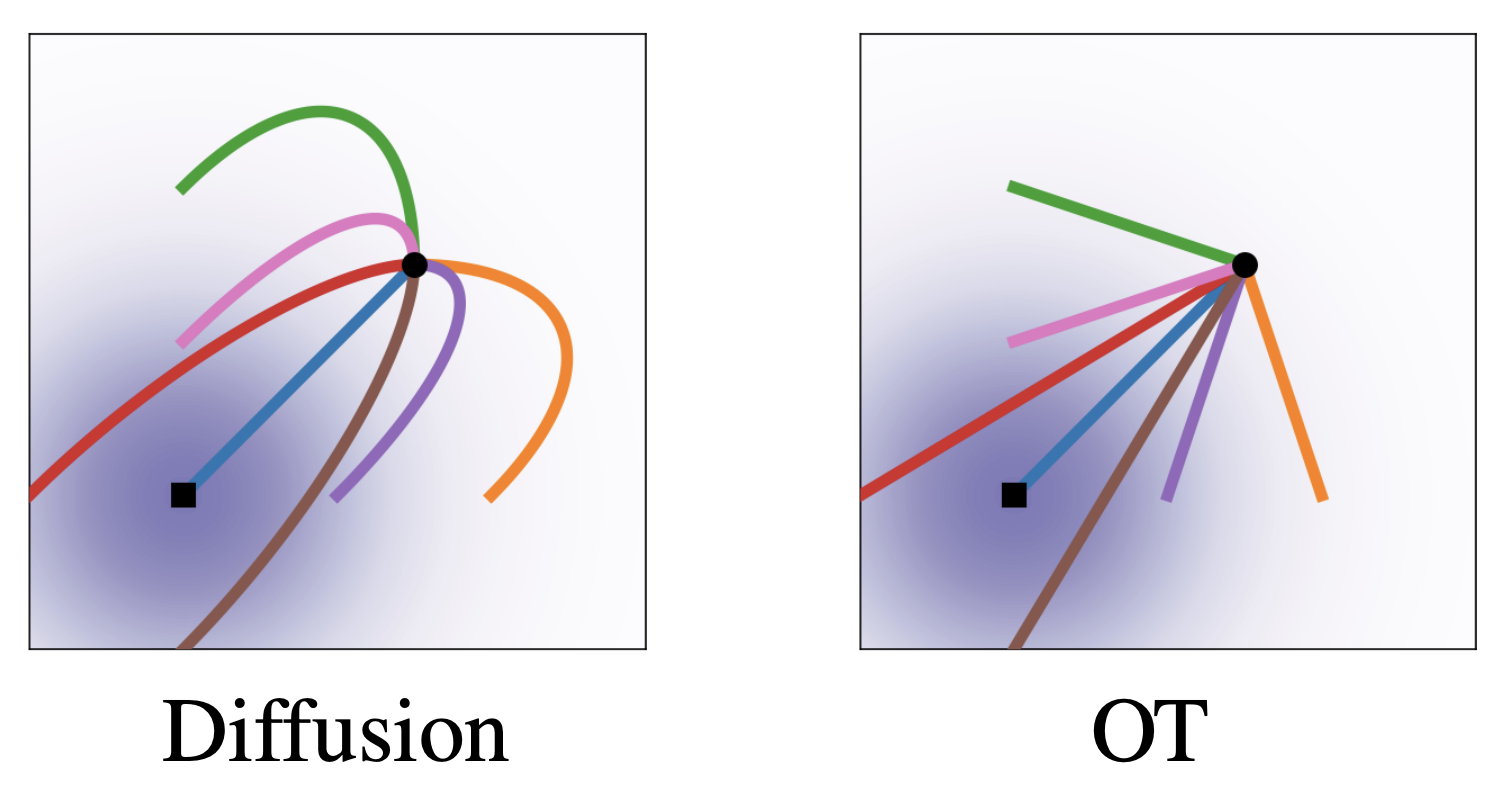
\includegraphics[width=0.6\linewidth]{figs/trajectories}
		\end{figure}
		\vspace{-0.3cm}
	\end{block}
	\begin{figure}
		\centering
		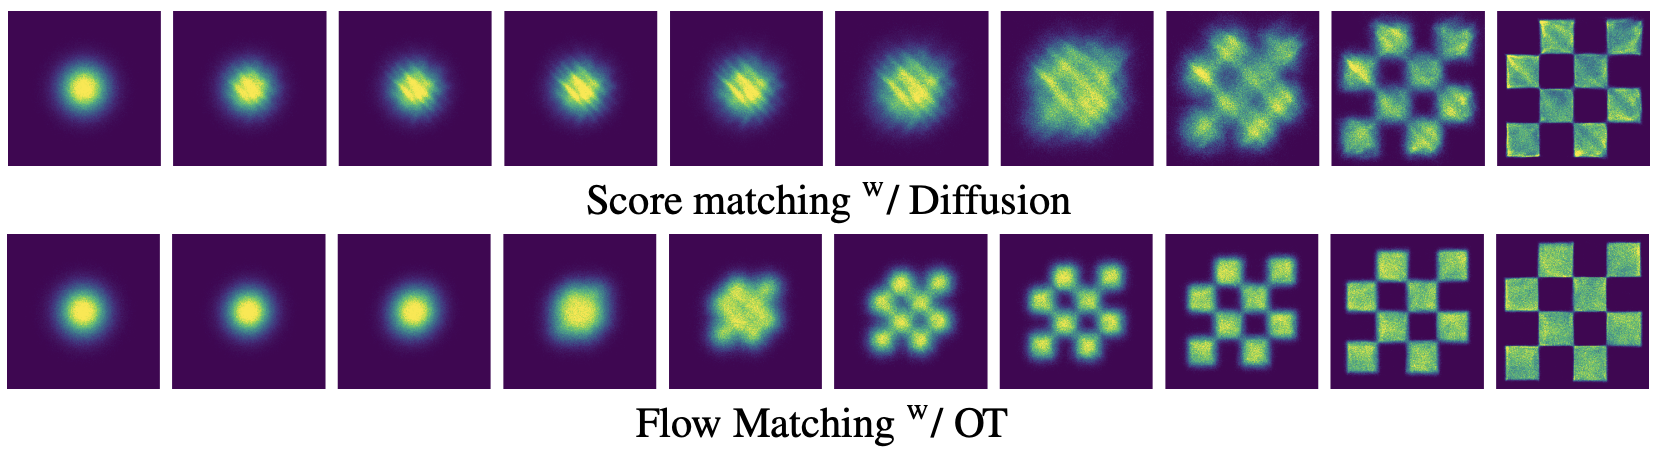
\includegraphics[width=\linewidth]{figs/2d-generation}
	\end{figure}
	\myfootnotewithlink{https://arxiv.org/abs/2210.02747}{Lipman Y., et al. Flow Matching for Generative Modeling, 2022}
\end{frame}
%=======
\begin{frame}{Summary}
	\begin{itemize}
		\item Conditional flow matching makes the FM objective tractable.
		\vfill
		\item Conical Gaussian paths serve as an effective FM technique.
		\vfill
		\item Pair conditioning yields the same procedure, but is more general (suitable for unpaired tasks).
		\vfill
		\item Diffusion and score-based models are special cases of the flow matching approach, but use curved trajectories.
	\end{itemize}
\end{frame}
\end{document}